\documentclass[spanish]{beamer}

% OPCIONES DE BEAMER

\definecolor{Maroon}{cmyk}{0, 0.87, 0.88, 0.1}
\definecolor{teal}{rgb}{0.0, 0.45, 0.45}

\usetheme[block=fill, subsectionpage=progressbar, titleformat section=smallcaps]{metropolis}
\setbeamertemplate{frametitle continuation}[roman]
\setbeamertemplate{section in toc}[balls numbered]
\setbeamertemplate{subsection in toc}[subsections unnumbered]
\widowpenalties 1 10000
\raggedbottom

% PAQUETES

\usepackage[utf8]{inputenc}
\usepackage[absolute,overlay]{textpos}
\usepackage[spanish, es-nodecimaldot]{babel}
\usepackage{microtype}
\usepackage{epigraph}
\usepackage{amssymb, amsmath, amsthm, amsfonts, amscd}
\usepackage{listings}
\usepackage{centernot}
\usepackage{caption}

% TÍTULO

\title{Análisis y modelado de series temporales con métodos estadísticos basados en Deep Learning}
\providecommand{\subtitle}[1]{}
\subtitle{Doble Grado en Ingeniería Informática y Matemáticas}
\date{\today}
\author{Miguel Lentisco Ballesteros}
\institute{Trabajo Fin de Grado \\\\\\ \textit{E.T.S de Ingenierías Informática y de Telecomunicación \\ Facultad de Ciencias}}

\titlegraphic{
  \begin{textblock*}{3cm}(8.5cm,5.8cm)
    
\includegraphics[width=3cm]{img/logo-ugr.png}
  \end{textblock*}
}
% DOCUMENTO

\begin{document}
\maketitle

\begin{frame}{Índice de contenidos}
  \tableofcontents[hideallsubsections]
\end{frame}

\section{Introducción y objetivos}

\begin{frame}{Introducción}
  En los últimos años se ha dado una extensa popularización y uso de las \textbf{redes neuronales} que ha dado lugar a una gran cantidad de trabajos de investigación diversos.\pause

  De aquí surge nuestra motivación de explorar en este campo ciertos temas que están \textbf{poco tratados} actualmente, en concreto, problemas con dominio de \textbf{series temporales} resueltos mediante redes neuronales \textbf{LSTM}.

  \pause

  Investigamos dos problemas de este tipo:
  \pause
  \begin{itemize}[<+->]
    \item \textbf{Selección de modelos} para clasificación de series temporales.
    \item \textbf{Detección de anomalías} en series temporales.
  \end{itemize}
\end{frame}

\begin{frame}{Objetivos}
  Los objetivos fundamentales de este proyecto son:
  \pause
  \begin{itemize}[<+->]
    \item Estudio y análisis del \textbf{marco teórico} relacionado con el campo del aprendizaje profundo, con hincapié en la arquitectura \textbf{LSTM}; y las \textbf{series temporales}, incluyendo las técnicas y modelos utilizados usualmente.
    \item Implementación y análisis del funcionamiento de una nueva heurística llamada \emph{Perturbation Validation} utilizada para la \textbf{selección} de modelos.
    \item Modelado y validación de un \textbf{detector} de series anómalas junto con el desarrollo de diversas \textbf{técnicas} que crean artificialmente series con perturbaciones.
  \end{itemize}
\end{frame}

\section{Conceptos base}

\subsection{Aprendizaje profundo}

\begin{frame}{Aprendizaje profundo}
  El \textbf{aprendizaje profundo} es el campo encargado de solucionar tareas del \textbf{aprendizaje automático} mediante el desarrollo de modelos basados en \textbf{redes neuronales}.
\end{frame}

\begin{frame}{Redes neuronales}
  Modelo \textbf{bioinspirado} en el sistema neuronal del cerebro.

  \pause

  La versión más simple y conocida es la \emph{feed-forward neural network} (FFNN).

  \begin{figure}
    \centering
    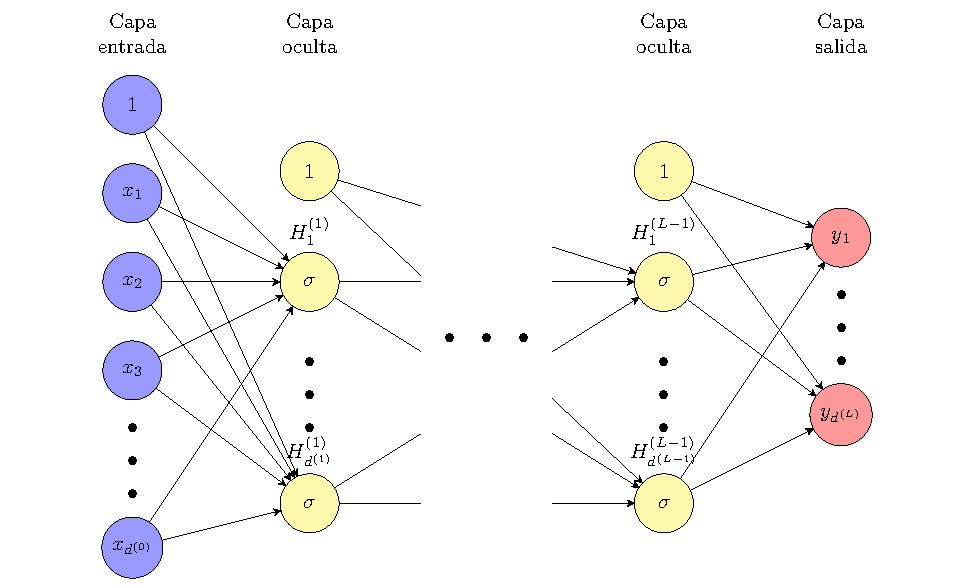
\includegraphics[width=0.6\textwidth]{img/ffnn}
    \caption{Estructura genérica de una \emph{feed-forward neural network}. Elaboración propia.}
  \end{figure}
\end{frame}

\begin{frame}{Desarrollo}
  En el trabajo se ha realizado un desarrollo de los siguientes apartados:
  \begin{itemize}
    \item Orígenes.
    \item Explicación y funcionamiento de la FFNN.
    \item Tipología y arquitecturas actuales. \textbf{LSTM}.
  \end{itemize}

\end{frame}

\begin{frame}{LSTM}
  La arquitectura LSTM (\emph{Long Short Term Memory}) es un tipo de red neuronal \textbf{recurrente} especializado para \textbf{datos secuenciales}, ya que de cada entrada se devuelve una salida y además cierta información que vuelve a la propia red, \textbf{retroalimentándose}, usada para la siguiente entrada.

  \begin{figure}
    \centering
    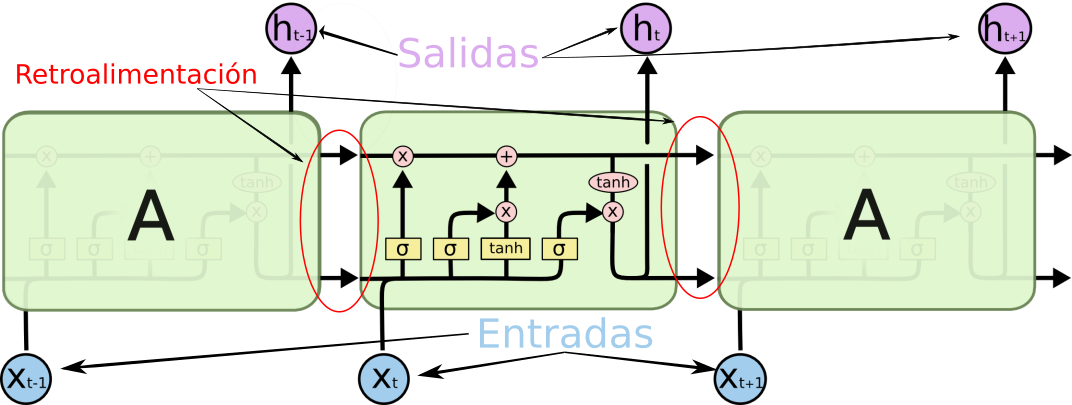
\includegraphics[width=0.8\textwidth]{img/lstm-cells}
    \caption{Esquema de funcionamiento de las neuronas LSTM. Extraído de \href{https://colah.github.io/posts/2015-08-Understanding-LSTMs/}{[enlace]}.}
  \end{figure}
\end{frame}

\subsection{Series temporales}

\begin{frame}{Definición}
  \begin{definition}[Proceso estocástico]
    Sean un espacio probabilístico $(\Omega, \mathcal{A}, P)$, un espacio Borel $(E, \mathcal{B}_E)$, un conjunto ordenado arbitrario $T$ y las variables aleatorias $X_t : (\Omega, \mathcal{A}, P) \to (E, \mathcal{B}_E), \; \forall t \in T$. Se dice que la familia de variables aleatorias ordenadas por $T$, $\{X_t\}_{t \in T}$, es un \textbf{proceso estocástico}.
  \end{definition}

  \pause

  \begin{definition}[Serie temporal]
    Sea un proceso estocástico $\{X_t\}_{t \in T}$, una \textbf{serie temporal} es una realización muestral del proceso, denotado por $\{x_t\}_{t \in T}$.
  \end{definition}
\end{frame}

\begin{frame}{Desarrollo}
  Se han desarrollado las siguientes partes:
  \begin{itemize}
    \item Teoría probabilística y de procesos estocásticos.
    \item Modelos estacionarios.
    \item \textbf{Descomposición} y diferenciación de series.
    \item Discretización de series.
  \end{itemize}
\end{frame}

\begin{frame}{Descomposición de series}
  Una técnica muy útil para el análisis de series es la \textbf{descomposición} en tres componentes esenciales:
  \pause
  \begin{itemize}[<+->]
    \item \textbf{Tendencia}: cambio en el nivel medio de la serie a largo plazo.
    \item \textbf{Estacionalidad}: patrón que se repite cada cierto periodo de tiempo.
    \item \textbf{Residuos}: valores sobrantes.
  \end{itemize}
  \pause[\thebeamerpauses]
  La descomposición se suele denotar como: $$x_t = m_t + s_t + Y_t, \; \forall t \in T,$$
  donde $m_t$ es la tendencia, $s_t$ es la estacionalidad e $Y_t$ los residuos.
\end{frame}

\begin{frame}{Descomposición STL}
  Una de las formas más usadas es la \textbf{descomposición STL} que solo necesita el periodo de la componente estacional.

  \begin{figure}
    \centering
    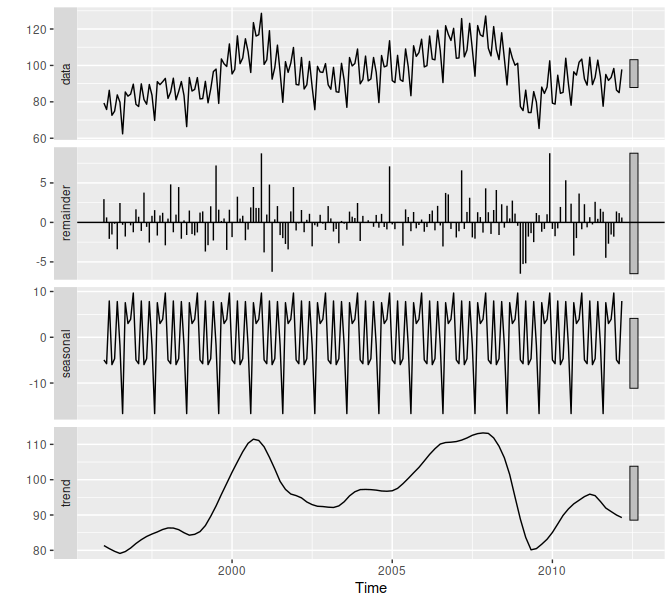
\includegraphics[width=0.55\textwidth]{img/stl-decomposition}
    \caption{Ejemplo de descomposición STL. Extraído de \cite{timeseries}.}
  \end{figure}
\end{frame}

\section{Selección de modelos}

\begin{frame}{Planteamiento}
  \textbf{Pregunta}: tengo varios modelos que han aprendido para resolver cierta tarea de clasificación de series temporales, ¿cual es el mejor?

  \pause

  \textbf{Respuesta}: el que tenga mejor acierto ($acc$).

  \pause

  \textbf{Problema}: sobreajuste.
\end{frame}

\begin{frame}{Selección clásica}
  \textbf{Solución}: dividir los datos en dos conjuntos: uno de entrenamiento y otro de \textbf{validación}. Seleccionamos en base al $acc$ en el conjunto de validación.

  \pause

  Se suele usar la \textbf{validación cruzada} para tener una mejor estimación.

  \begin{figure}
    \centering
    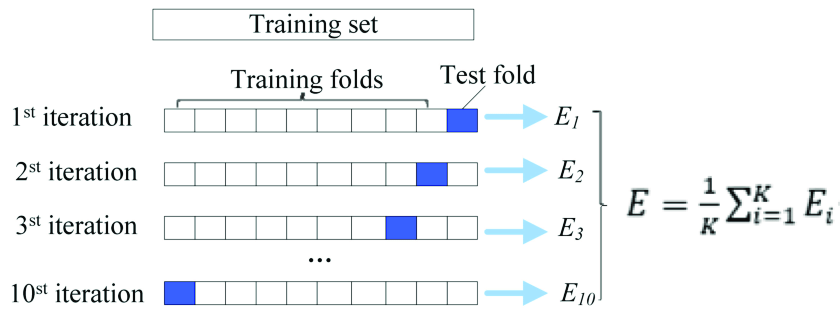
\includegraphics[width=.8 \textwidth]{img/cv}
    \caption{Esquema de validación cruzada. Extraído de \href{https://www.semanticscholar.org/paper/RFAmyloid\%3A-A-Web-Server-for-Predicting-Amyloid-Niu-Li/bf91ead8b0d49922dab952aa7f96e1480578289c/figure/6}{[enlace]}.}
  \end{figure}
\end{frame}

\begin{frame}{Problemas de la validación}
  \textbf{Inconvenientes}:
  \begin{itemize}
    \item Datos de validación insuficientes para representar la distribución subyacente.
    \item Sesgo en la muestra.
    \item No tiene en cuenta la complejidad.
  \end{itemize}
\end{frame}

\subsection{Perturbation Validation}

\begin{frame}{Perturbated Validation}
  \emph{Perturbation Validation} ($PV$) es una heurística que evalúa el ajuste del modelo frente a su espacio de hipótesis, midiendo el nivel de cambio del $acc$ al introducir etiquetas erróneas.

  \pause

  Si el modelo ha aprendido correctamente el patrón subyacente en los datos, no sobreajustará las etiquetas incorrectas.

  \pause

  Tiene en cuenta el ajuste y la complejidad del modelo sin tener que realizar una partición de los datos.
\end{frame}


\begin{frame}{Obtención}
  1. Se crean $k$ conjuntos de etiquetas perturbadas en base a unos ratios de error $r_i, \, i = 1, \ldots, k$.
  \pause

  2. Para cada conjunto de etiquetas, el modelo se entrena desde cero con dicho conjunto y se evalua el ajuste con los mismos datos, obteniendo $acc_i, \, i = 1, \ldots, k$.
  \pause

  3. $PV$ es la pendiente absoluta de la regresión lineal obtenida con los puntos $\{(r_i, acc_i)\}_{i = 1}^k$.
\end{frame}

\begin{frame}{Funcionamiento}
  \begin{figure}
    \centering
    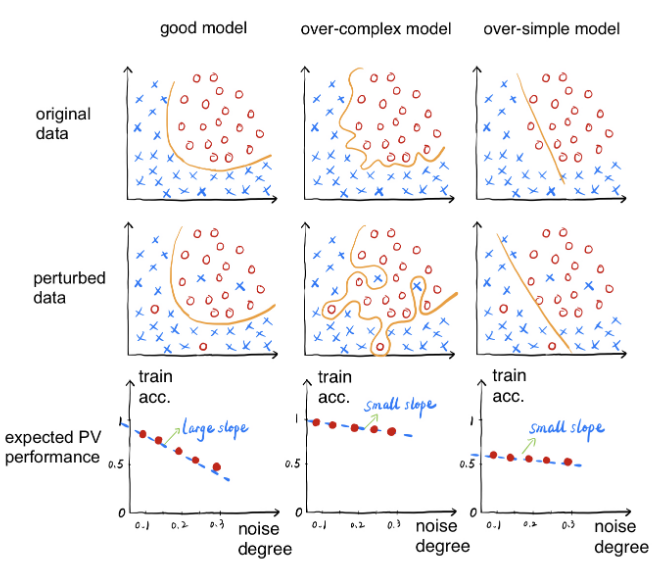
\includegraphics[width=.6\textwidth]{img/idea-pv}
    \caption{Idea de funcionamiento del PV. Extraído de \cite{pv}}
  \end{figure}
\end{frame}

\subsection{Experimentación}

\begin{frame}{Descripción}
  Realizamos el siguiente experimento para medir la eficacia del $PV$:
  \begin{itemize}
    \item 114 \emph{datasets} de series temporales unidimensionales de tareas de clasificación, divididos en entrenamiento y test.
    \item 11 modelos de clasificación usuales: nuestro modelo LSTM, SVM, $k$-NN y distintos árboles.
    \item Métricas medidas: $PV$, $acc_{5\textemdash CV}$, $acc_{train}$, $acc_{test}$.
  \end{itemize}
\end{frame}

\begin{frame}{Resultados}
  \begin{figure}
    \centering
    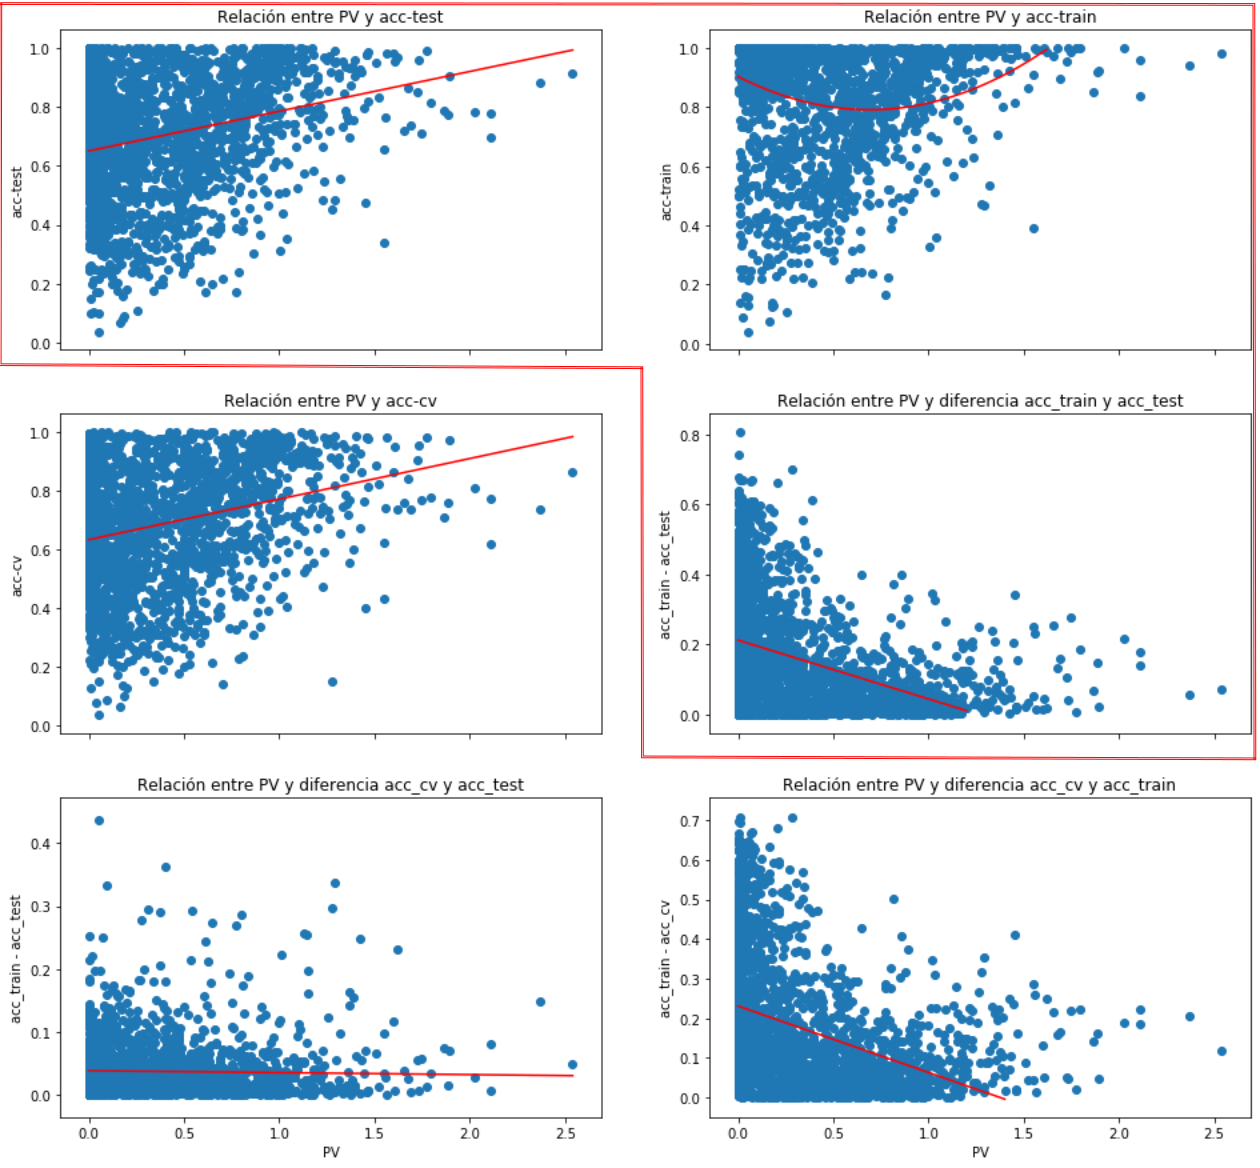
\includegraphics[width=.74\textwidth]{img/res-pv}
    \caption{Resultados del experimento. Elaboración propia.}
  \end{figure}
\end{frame}

\begin{frame}{Análisis}
  Concluímos que:
  \begin{itemize}
    \item $PV \uparrow \implies E[acc_{train}]\uparrow, E[acc_{test}] \uparrow$.
    \item $PV$ es inversamente proporcional al sobreajuste.
  \end{itemize}
  \pause

  Pero...
  \begin{itemize}
    \item $PV(clf_1) > PV(clf_2) \centernot\Longrightarrow acc_{test}(clf_1) > acc_{test}(clf_2)$.
    \item Los modelos con alta varianza (LSTM) producen valores atípicos.
  \end{itemize}

\end{frame}

\begin{frame}{Complementación}
  PV no \textbf{sustituye} a $acc_{CV}$ pero puede \textbf{complementarlo}:
  \begin{enumerate}
    \item Seleccionamos los modelos con $acc_{CV}$ más altos.
    \item Calculamos el PV para estos modelos.
    \item Escogemos el modelo con PV más alto si $PV >> 0$.
  \end{enumerate}
\end{frame}

\begin{frame}{Hiperparámetros}
  \begin{figure}
    \centering
    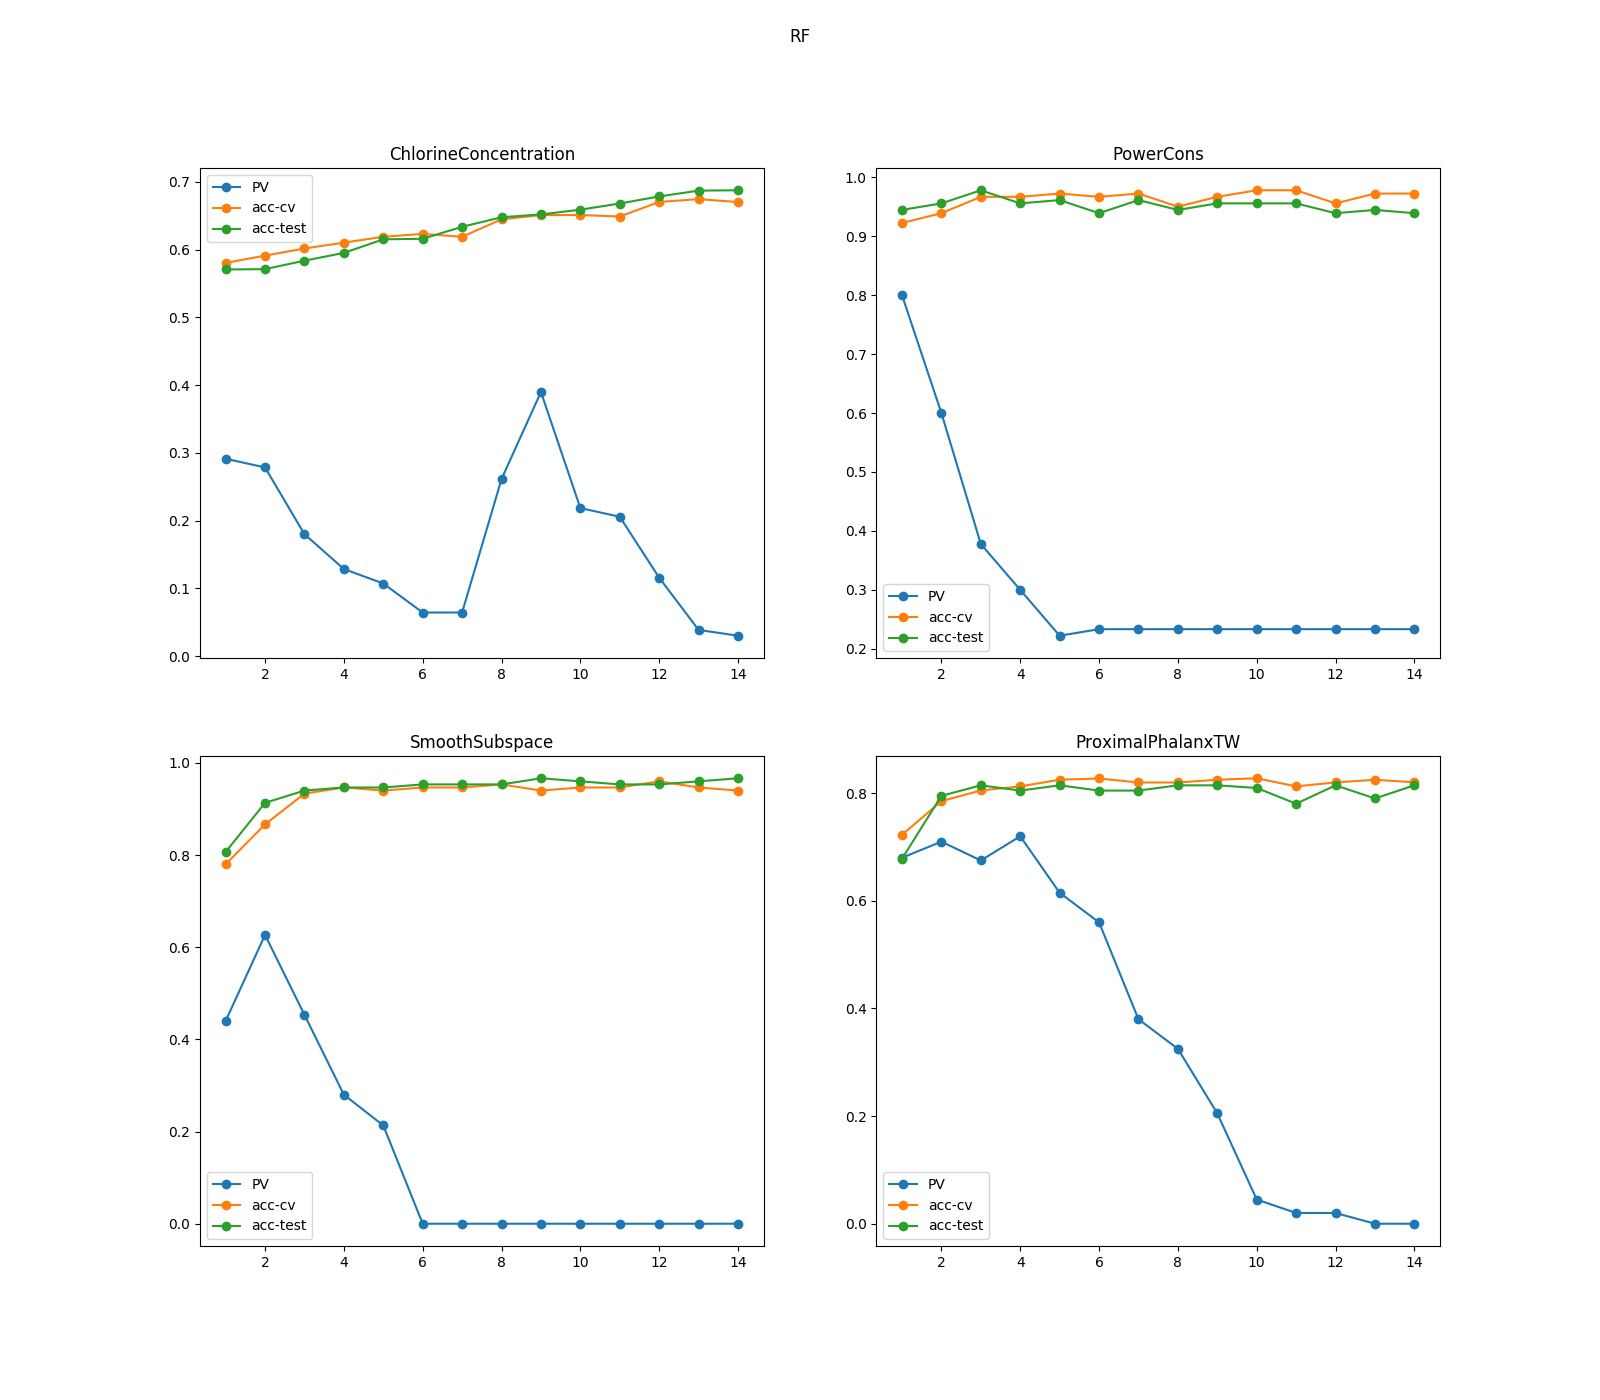
\includegraphics[width=.78\textwidth]{img/hiper-RF}
    \caption{Experimento con hiperparámetros. Elaboración propia.}
  \end{figure}
\end{frame}

\section{Detección de anomalías}

\begin{frame}{Anomalías}
  Una serie temporal es \textbf{anómala} cuando se producen valores inesperados en ciertos instantes. \pause Aunque dependen de la tarea concreta existen ciertos tipos usuales: cambios de intensidad puntuales o en un periodo, cambio de forma...
  \pause

  Abordamos dos problemas en este campo:
  \begin{itemize}
    \item Falta de detectores desplegables en \textbf{diversas} tareas.
    \item Falta de \emph{datasets} con muestras de series anómalas.
  \end{itemize}
\end{frame}

\subsection{Detector}

\begin{frame}{Estructura}
  Modelamos un detector de series anómalas extensible para muchos casos, estructurado en dos partes:

  \begin{itemize}
    \item \emph{Autoencoder} LSTM para reconstrucción.
    \item Predictor basado en la distribución de los errores.
  \end{itemize}
\end{frame}

\begin{frame}{Autoencoder LSTM}
  Un \emph{autoencoder} LSTM que aprende el \textbf{patrón} de las series normales. Reconstruye las entradas para el patrón aprendido.

  \begin{figure}[ht]
    \centering
    \begin{minipage}[b]{.45\textwidth}
      \centering
      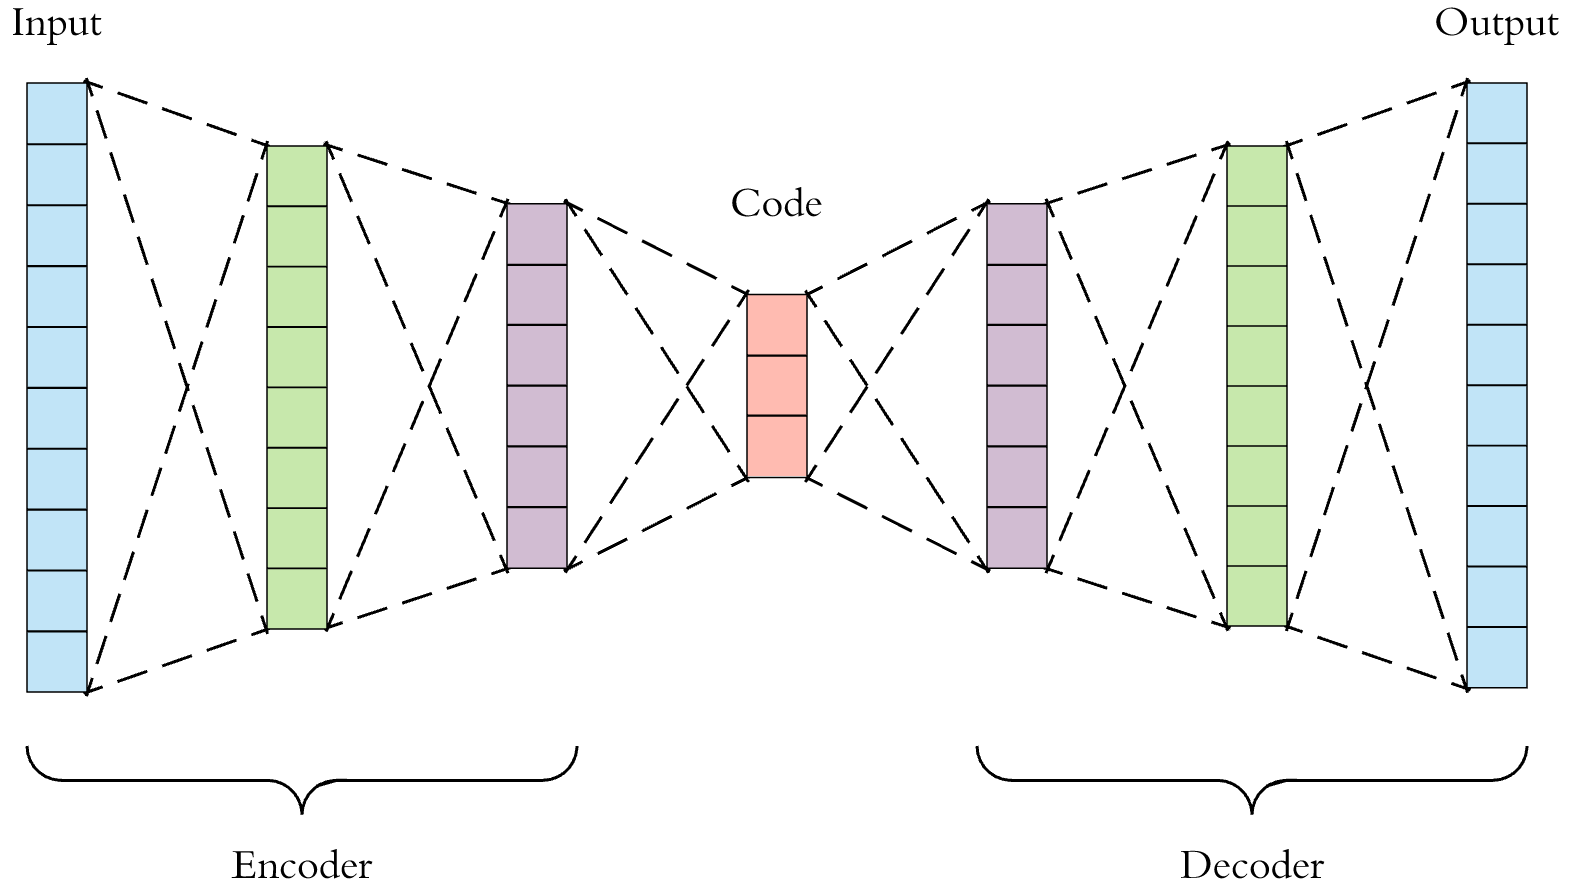
\includegraphics[width=1\linewidth]{img/ae}
      \caption{Arquitectura autoencoder. Extraído de \href{http://www.cs.us.es/~fsancho/?e=232}{[enlace]}.}
    \end{minipage}
    \hspace{0.5cm}
    \begin{minipage}[b]{.45\textwidth}
      \centering
      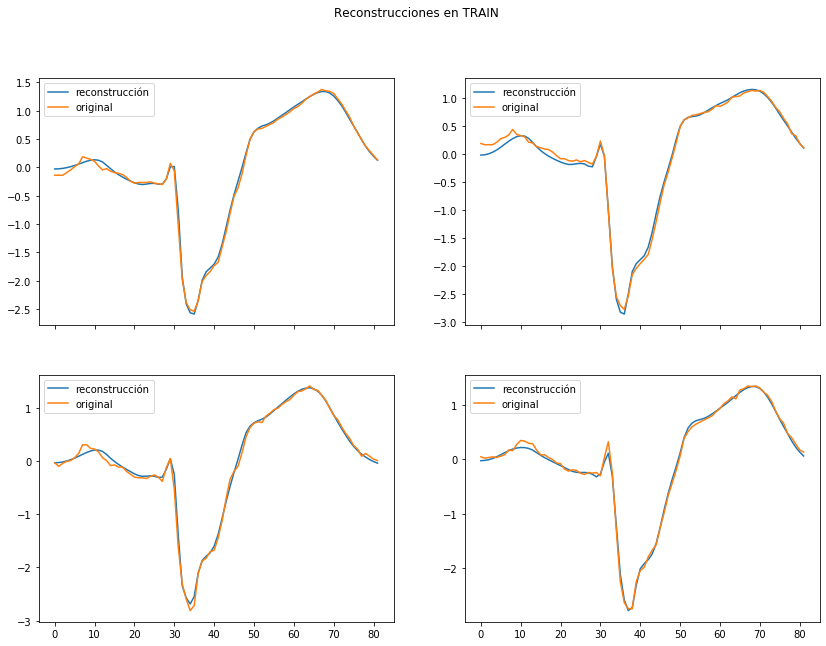
\includegraphics[width=1\linewidth]{img/ae-reconstruccion}
      \caption{Ejemplos de reconstrucciones. Elaboración propia.}
    \end{minipage}
  \end{figure}
\end{frame}

\begin{frame}{Predictor}
  Probabilidad de anomalía asignada en base a la \textbf{distribución} aprendida de los errores cuadráticos medios entre las series normales y las reconstrucciones.

  \begin{figure}
    \centering
    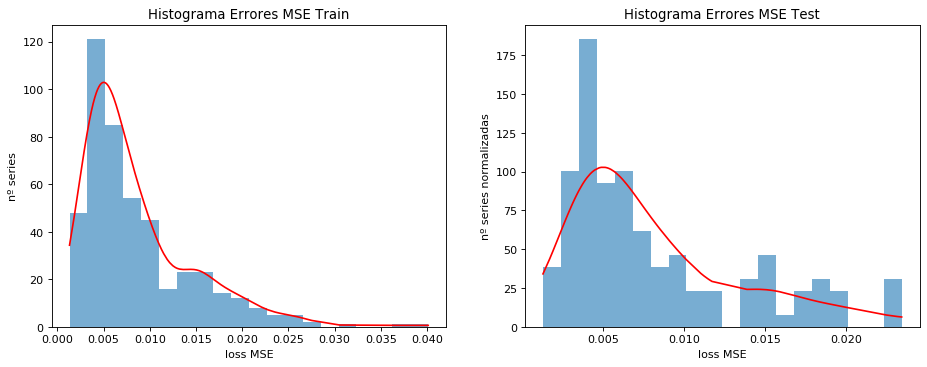
\includegraphics[width=1\linewidth]{img/hists}
    \caption{Ejemplo de distribución de errores. Elaboración propia.}
  \end{figure}
\end{frame}

\subsection{Alteraciones}

\begin{frame}{Alteraciones}
  Cuatro métodos para alterar series normales que permiten:
  \begin{itemize}
    \item Validar detectores de anomalías cuando solo hay series normales.
    \item Crear muestras anómalas de entrenamiento para clasificadores.
  \end{itemize}
  \pause

  Siempre se selecciona un tramo aleatorio de la serie y se modifica.
\end{frame}

\begin{frame}{Ruido gaussiano}
  Simulamos cambios grandes puntuales en la intensidad de la serie (\emph{picos}) mediante \textbf{distribución gaussiana}.

  \begin{figure}
    \centering
    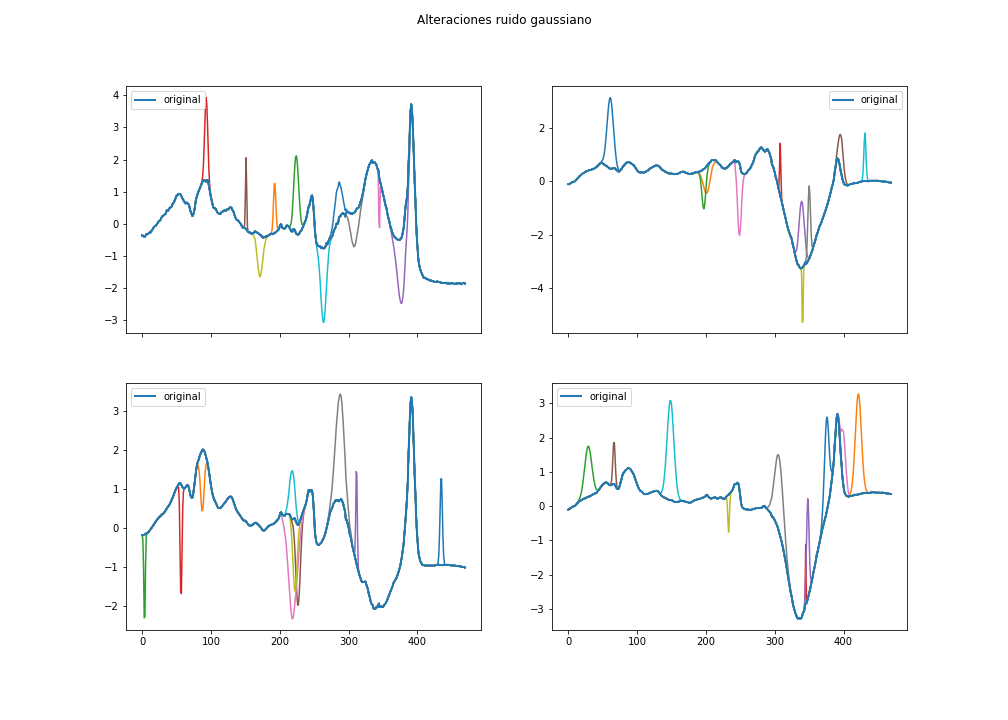
\includegraphics[width=.8\linewidth]{img/ruido-gauss}
    \caption{Perturbaciones con ruido gaussiano. Elaboración propia.}
  \end{figure}
\end{frame}

\begin{frame}{Pulso gaussiano-sinusoidal}
  Simulamos cambios de forma o interferencias en las series mediante un \textbf{pulso gaussiano-sinusoidal}.

  \begin{figure}
    \centering
    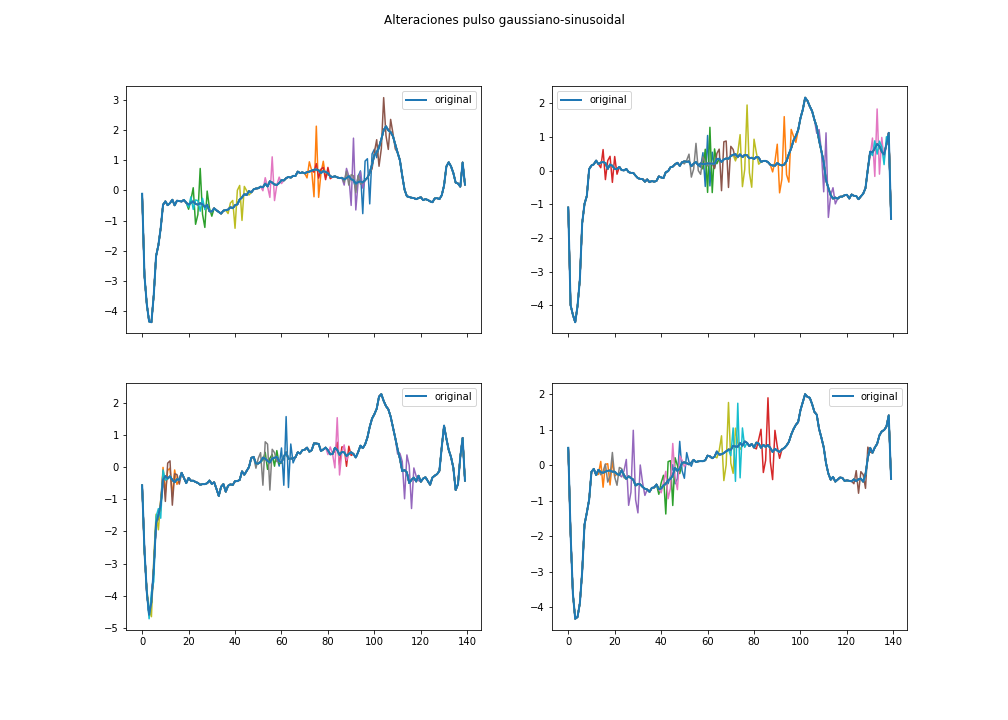
\includegraphics[width=.8\linewidth]{img/pulso-gaussinus}
    \caption{Alteraciones pulso g.s. Elaboración propia.}
  \end{figure}
\end{frame}

\begin{frame}{Intensidad estacionalidad}
  Simulamos cambios estacionales alterando la intensidad de la \textbf{estacionalidad} de la serie.

  \begin{figure}
    \centering
    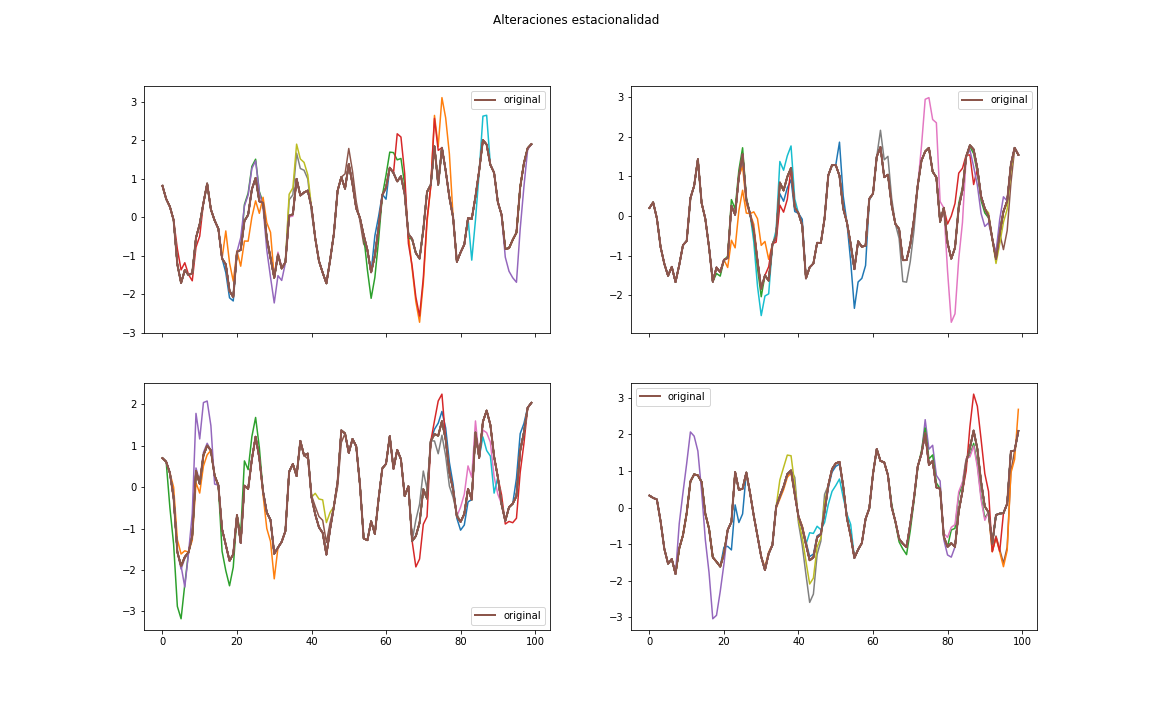
\includegraphics[width=.92\linewidth]{img/estacionalidad}
    \caption{Perturbaciones con estacionalidad. Elaboración propia.}
  \end{figure}
\end{frame}

\begin{frame}{Intensidad tendencia}
  Simulamos cambios estacionales alterando la intensidad de la \textbf{tendencia} de la serie.

  \begin{figure}
    \centering
    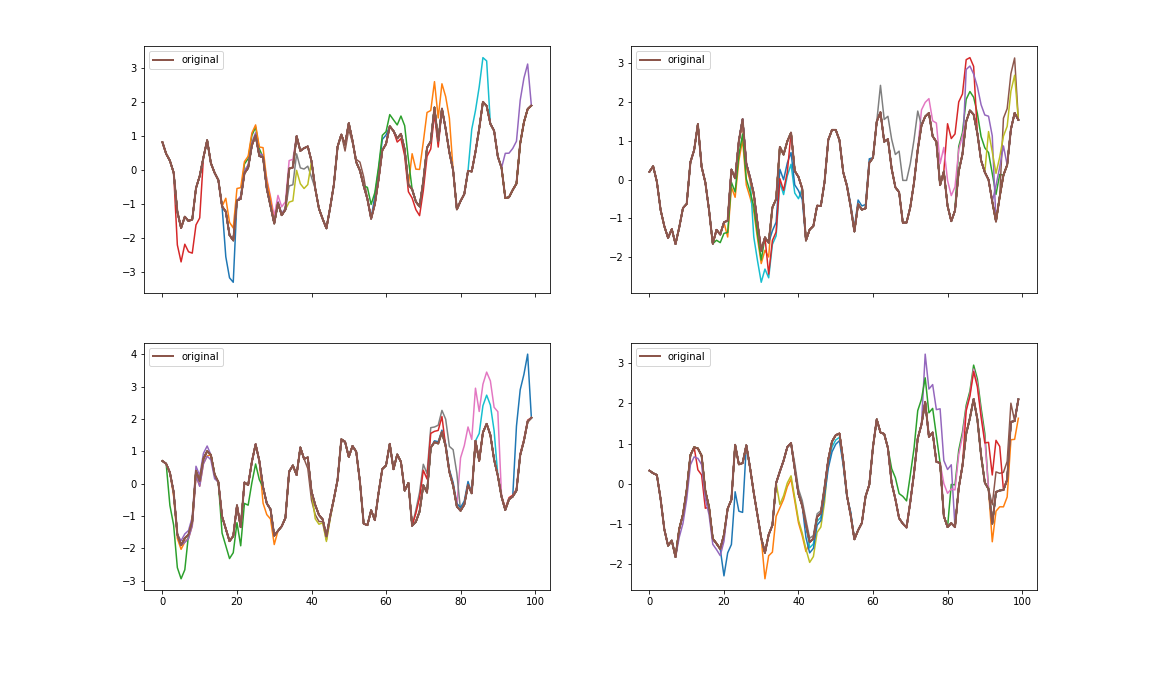
\includegraphics[width=.92\linewidth]{img/tendencia}
    \caption{Perturbaciones con tendencia. Elaboración propia.}
  \end{figure}
\end{frame}

\subsection{Experimentación}

\begin{frame}{Descripción}
  Validamos empíricamente la eficacia del detector para cada método de alteración propuesto en un par de \emph{datasets} sin muestras anómalas.
  \pause

  Probamos con distintos parámetros para crear las series anómalas y observamos el cambio de comportamiento del detector frente a los distintos valores tomados.
\end{frame}

\begin{frame}{Resultados}
  En general hemos observado que:
  \begin{itemize}
    \item El detector consigue unos buenos resultados de la métrica.
    \item Las alteraciones se comportan adecuadamente.
  \end{itemize}

  \begin{figure}
    \centering
    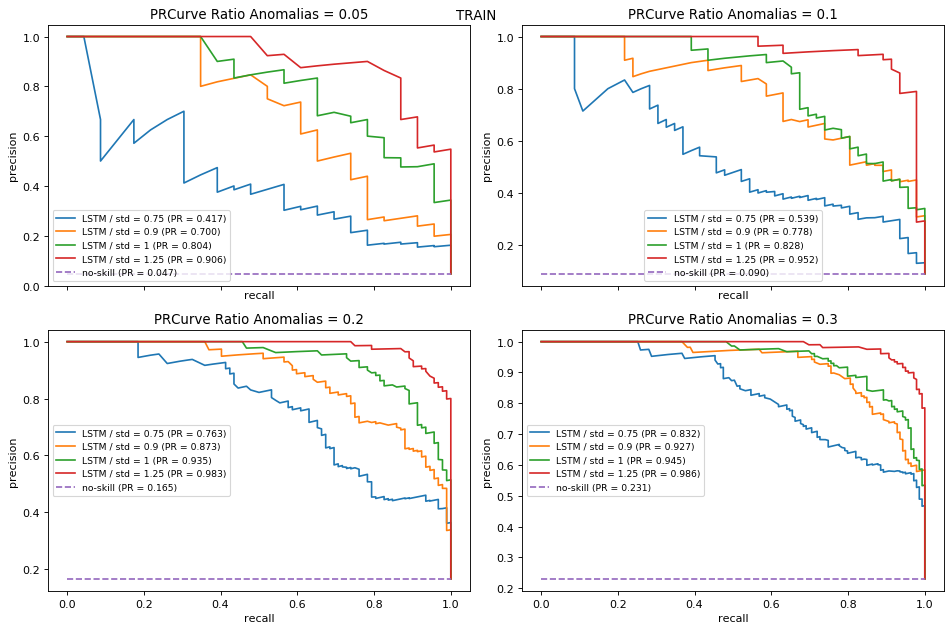
\includegraphics[width=.68\linewidth]{img/validacion}
    \caption{Ejemplo de validación del detector. Elaboración propia.}
  \end{figure}
\end{frame}

\begin{frame}{Conclusiones}
  En este trabajo hemos logrado:
  \pause
  \begin{itemize}[<+->]
    \item Estudiar con detalle el marco teórico actual de las redes neuronales y las series temporales.
    \item Analizar y comprobar la efectividad de \emph{Perturbation Validation}, que puede complementar el método clásico de selección de modelos.
    \item Modelar un detector de series anómalas efectivo y fácil de desplegar en diversas tareas, junto con métodos para crear muestras anómalas para su uso en validación o entrenamiento.
  \end{itemize}
\end{frame}

\begin{frame}{Referencias}
  \begin{thebibliography}{9}
    \bibitem{deeplearning-1} \textsc{Abu-Mostafa, Y. S., Magdon-Ismail, M. \& Lin, H. T}. (2012). \textit{Learning from data}.
    \bibitem{deeplearning-2} \textsc{Goodfellow, I., Bengio, Y. \& Courville, A}. (2016). \textit{Deep Learning}.
    \bibitem{timeseries} \textsc{Hyndman, R. J. \& Athanasopoulos, G}. (2018). \textit{Forecasting: principles and practice}.
    \bibitem{pv} \textsc{Zhang, J. M., Harman, M., Guedj, B., Barr, E. T. \& Shawe-Taylor, J}. (2019). \textit{Perturbation validation: a new heuristic to validate machine learning models}.
    \bibitem{anomaly} \textsc{Ahmed, M., Mahmood, A. N. \& Hu, J}. (2016). \textit{A survey of network anomaly detection techniques}.
  \end{thebibliography}
\end{frame}

\begin{frame}[standout]
  Gracias por su atención.
\end{frame}

\end{document}
